% Alur teknis SeBatt: rantai perangkat dan urutan protokol saat penukaran.
% Versi untuk slide: kanvas 16:9, teks besar, kode status diambil dari spesifikasi.md.
% Kompilasi: tectonic -X compile alur-teknis.tex  (atau latexmk -pdf alur-teknis.tex)
% PNG: pdftoppm -png -r 300 -singlefile alur-teknis.pdf alur-teknis
\documentclass[border=10pt]{standalone}
\usepackage[T1]{fontenc}
\usepackage[scaled=0.92]{helvet}
\renewcommand{\familydefault}{\sfdefault}
\usepackage{tikz}
\usetikzlibrary{positioning,arrows.meta,calc}

\definecolor{ok}{HTML}{16A34A}
\definecolor{bad}{HTML}{DC2626}
\newcommand{\sub}[1]{{\small #1}}

\begin{document}
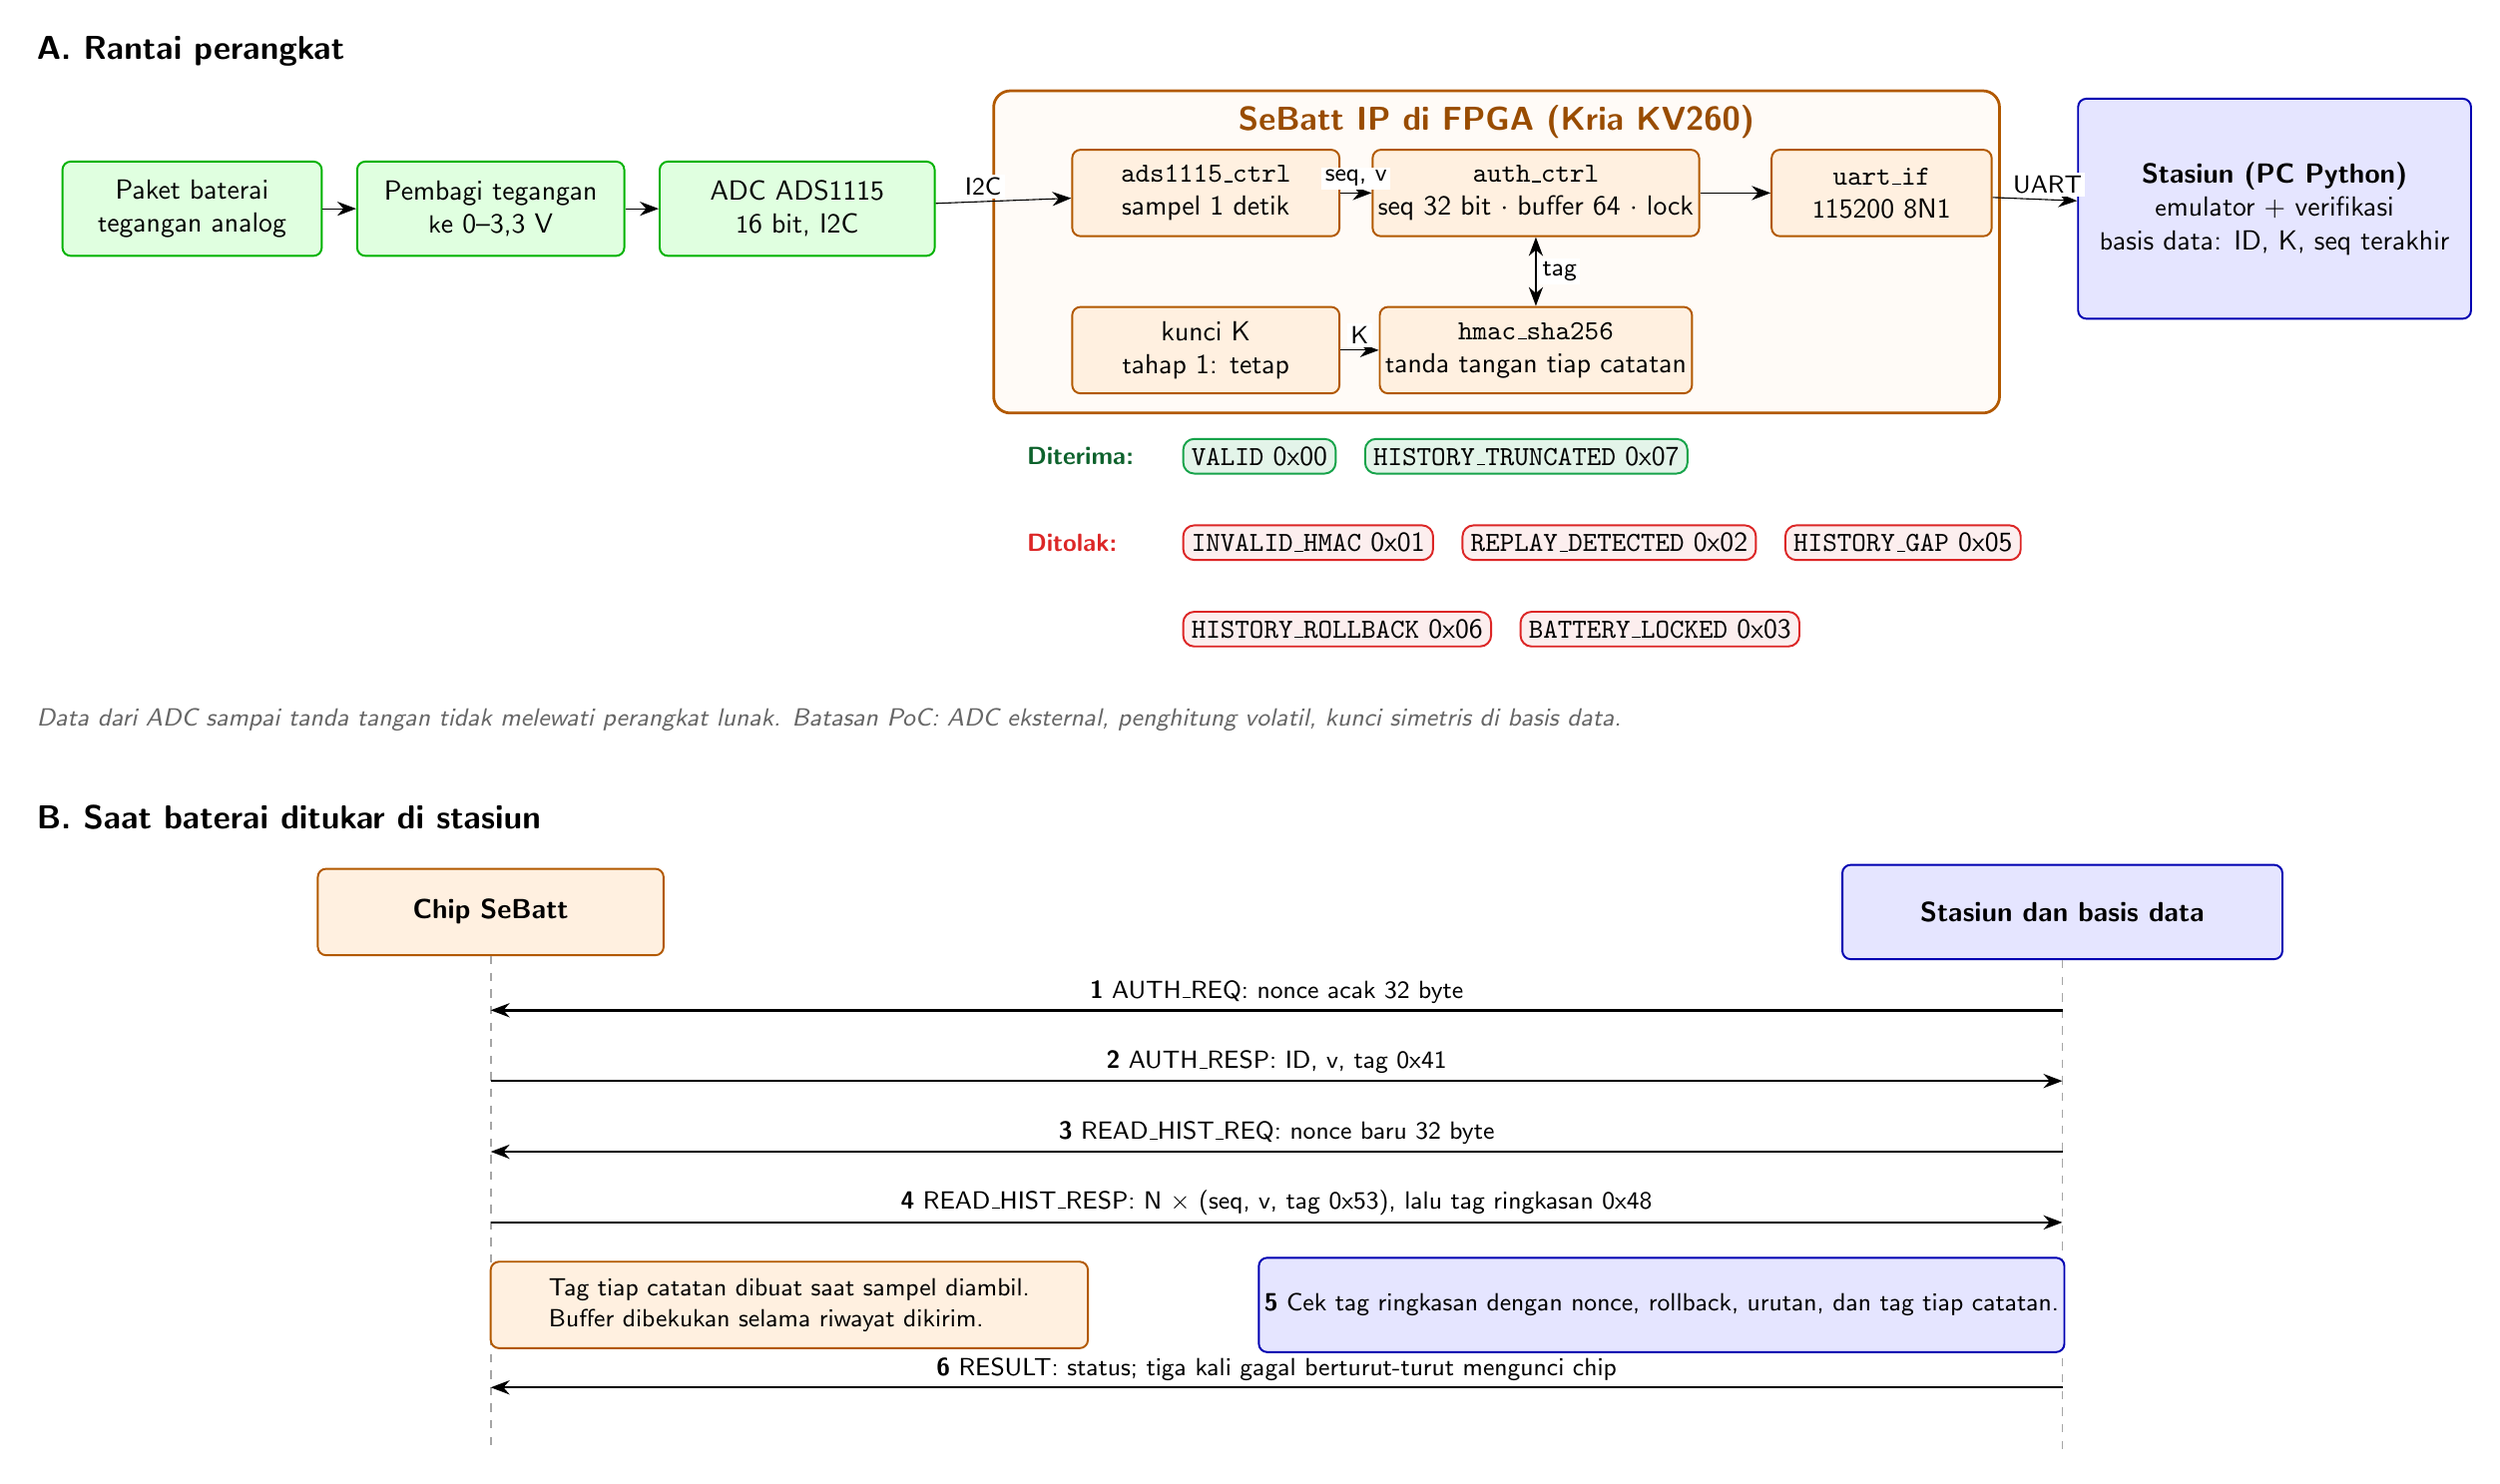
\begin{tikzpicture}[
    font=\normalsize, >={Stealth[length=2.4mm]},
    src/.style={draw=green!70!black, fill=green!12, rounded corners=3pt, align=center,
                line width=0.7pt, minimum height=1.2cm, inner sep=2pt},
    ipl/.style={draw=orange!70!black, fill=orange!12, rounded corners=3pt, align=center,
                line width=0.7pt, minimum height=1.1cm, inner sep=2pt},
    stn/.style={draw=blue!70!black, fill=blue!10, rounded corners=3pt, align=center,
                line width=0.7pt, minimum height=1.2cm, inner sep=2pt},
    chipG/.style={draw=ok, fill=ok!12, rounded corners=4pt, line width=0.7pt,
                  align=center, inner sep=3pt},
    chipB/.style={draw=bad, fill=bad!8, rounded corners=4pt, line width=0.7pt,
                  align=center, inner sep=3pt},
    lbl/.style={font=\small, fill=white, inner sep=1.2pt},
    title/.style={font=\bfseries\large, anchor=west},
    msg/.style={->, line width=0.9pt}
  ]

  % =====================================================================
  % A. Rantai perangkat
  % =====================================================================
  \node[title] at (-0.4,5.5) {A. Rantai perangkat};

  % Kotak IP (digambar lebih dulu supaya node di atasnya)
  \draw[orange!70!black, fill=orange!3, rounded corners=6pt, line width=1pt]
    (11.9,5.0) rectangle (24.7,0.9);
  \node[font=\bfseries\large, text=orange!60!black] at (18.3,4.6) {SeBatt IP di FPGA (Kria KV260)};

  % Sumber analog
  \node[src, minimum width=3.3cm] (bat) at (1.7,3.5) {Paket baterai\\{\sub tegangan analog}};
  \node[src, minimum width=3.4cm] (div) at (5.5,3.5) {Pembagi tegangan\\{\sub ke 0--3,3 V}};
  \node[src, minimum width=3.5cm] (adc) at (9.4,3.5) {ADC ADS1115\\{\sub 16 bit, I2C}};

  % Isi IP
  \node[ipl, minimum width=3.4cm] (adcif) at (14.6,3.7) {\texttt{ads1115\_ctrl}\\{\sub sampel 1 detik}};
  \node[ipl, minimum width=3.6cm] (ctrl)  at (18.8,3.7) {\texttt{auth\_ctrl}\\{\sub seq 32 bit $\cdot$ buffer 64 $\cdot$ lock}};
  \node[ipl, minimum width=2.8cm] (uart)  at (23.2,3.7) {\texttt{uart\_if}\\{\sub 115200 8N1}};
  \node[ipl, minimum width=3.4cm] (key)   at (14.6,1.7) {kunci K\\{\sub tahap 1: tetap}};
  \node[ipl, minimum width=3.6cm] (hmac)  at (18.8,1.7) {\texttt{hmac\_sha256}\\{\sub tanda tangan tiap catatan}};

  % Stasiun
  \node[stn, minimum width=5.0cm, minimum height=2.8cm] (st) at (28.2,3.5)
    {\textbf{Stasiun (PC Python)}\\{\sub emulator + verifikasi}\\{\sub basis data: ID, K, seq terakhir}};

  % Tanda panah rantai
  \draw[->] (bat) -- (div);
  \draw[->] (div) -- (adc);
  \draw[->] (adc) -- node[lbl, above=1pt, pos=0.35]{I2C} (adcif);
  \draw[->] (adcif) -- node[lbl, above=1pt]{seq, v} (ctrl);
  \draw[->] (ctrl) -- (uart);
  \draw[->] (uart) -- node[lbl, above=1pt, pos=0.65]{UART} (st);
  \draw[<->] (ctrl) -- node[lbl, midway, right=1pt]{tag} (hmac);
  \draw[->] (key) -- node[lbl, above=1pt]{K} (hmac);

  % Kode status (hasil keputusan stasiun)
  \node[font=\small\bfseries, text=ok!60!black, anchor=west] at (12.2,0.35) {Diterima:};
  \node[chipG, anchor=west] (s1) at (14.3,0.35) {\texttt{VALID} 0x00};
  \node[chipG, right=0.35cm of s1] {\texttt{HISTORY\_TRUNCATED} 0x07};

  \node[font=\small\bfseries, text=bad, anchor=west] at (12.2,-0.75) {Ditolak:};
  \node[chipB, anchor=west] (s2) at (14.3,-0.75) {\texttt{INVALID\_HMAC} 0x01};
  \node[chipB, right=0.35cm of s2] (s3) {\texttt{REPLAY\_DETECTED} 0x02};
  \node[chipB, right=0.35cm of s3] {\texttt{HISTORY\_GAP} 0x05};
  \node[chipB, anchor=west] (s4) at (14.3,-1.85) {\texttt{HISTORY\_ROLLBACK} 0x06};
  \node[chipB, right=0.35cm of s4] {\texttt{BATTERY\_LOCKED} 0x03};

  \node[font=\small\itshape, text=black!60, anchor=west] at (-0.4,-3.0)
    {Data dari ADC sampai tanda tangan tidak melewati perangkat lunak.
     Batasan PoC: ADC eksternal, penghitung volatil, kunci simetris di basis data.};

  % =====================================================================
  % B. Urutan protokol saat penukaran
  % =====================================================================
  \node[title] at (-0.4,-4.25) {B. Saat baterai ditukar di stasiun};

  \node[ipl, minimum width=4.4cm] (chip) at (5.5,-5.45) {\textbf{Chip SeBatt}};
  \node[stn, minimum width=5.6cm] (srv) at (25.5,-5.45) {\textbf{Stasiun dan basis data}};

  \draw[black!35, dashed, line width=0.6pt] (chip.south) -- ++(0,-6.3);
  \draw[black!35, dashed, line width=0.6pt] (srv.south) -- ++(0,-6.3);

  \draw[msg] (25.5,-6.7) -- node[lbl, above=1pt]{\textbf{1} AUTH\_REQ: nonce acak 32 byte} (5.5,-6.7);
  \draw[msg] (5.5,-7.6) -- node[lbl, above=1pt]{\textbf{2} AUTH\_RESP: ID, v, tag 0x41} (25.5,-7.6);
  \draw[msg] (25.5,-8.5) -- node[lbl, above=1pt]{\textbf{3} READ\_HIST\_REQ: nonce baru 32 byte} (5.5,-8.5);
  \draw[msg] (5.5,-9.4) -- node[lbl, above=1pt]{\textbf{4} READ\_HIST\_RESP: N $\times$ (seq, v, tag 0x53), lalu tag ringkasan 0x48} (25.5,-9.4);
  \draw[msg] (25.5,-11.5) -- node[lbl, above=1pt]{\textbf{6} RESULT: status; tiga kali gagal berturut-turut mengunci chip} (5.5,-11.5);

  \node[ipl, minimum width=7.6cm, align=left, font=\small] (tagm) at (9.3,-10.45)
    {Tag tiap catatan dibuat saat sampel diambil.\\Buffer dibekukan selama riwayat dikirim.};
  \node[stn, minimum width=10.2cm, align=left, font=\small] (cek) at (20.4,-10.45)
    {\textbf{5} Cek tag ringkasan dengan nonce, rollback, urutan, dan tag tiap catatan.};

\end{tikzpicture}
\end{document}
